% 【拆分生成】 answers.tex —— 2018 年·全国Ⅰ卷·理科 · 参考答案与详细解析片段
% 【拆分生成】 由 tools/split_project.py 自合并书 answers/2018_g1_li_sol.tex 包裹 answer 环境生成，勿手改
% 由 tools/md2tex.py 自 2018_数学真题_理_含解析.md 生成，勿手改（改源 MD 后重跑）


\begin{gknotice}
\textbf{ 解析归属声明}：本文解析由本库编写者根据试题\textbf{独立推导}，\textbf{非官方标准答案}。若与官方发布版本不一致，以官方为准。

\textbf{ 卷种提示}：本卷为文理分科时代的旧结构，含\textbf{现已取消}的选做题（第 22/23 题）与\textbf{已删除}的三视图考点（第 7 题）。
\end{gknotice}

\par\medskip

\gkpart{一、选择题}

\begin{answer}
\gksolhead{1}{复数运算}

\textbf{题目}：设 $z=\dfrac{1-\mathrm i}{1+\mathrm i}+2\mathrm i$，则 $|z|=$（　　）A．$0$　B．$\dfrac12$　C．$1$　D．$\sqrt2$

\textbf{解析}

先化简分式。分子分母同乘 $(1-\mathrm i)$：

\[\frac{1-\mathrm i}{1+\mathrm i}=\frac{(1-\mathrm i)^{2}}{(1+\mathrm i)(1-\mathrm i)}=\frac{1-2\mathrm i+\mathrm i^{2}}{1-\mathrm i^{2}}=\frac{-2\mathrm i}2=-\mathrm i\]

于是

\[z=-\mathrm i+2\mathrm i=\mathrm i,\qquad |z|=1\]

\gkanswer{答案：C}

\begin{gktip}
\textbf{方法提示}：$\dfrac{1-\mathrm i}{1+\mathrm i}=-\mathrm i$ 与 $\dfrac{1+\mathrm i}{1-\mathrm i}=\mathrm i$ 值得记住，考场上省下一步计算。
\end{gktip}

\par\medskip

\end{answer}
\begin{answer}
\gksolhead{2}{一元二次不等式与补集}

\textbf{题目}：$A=\left\{x\mid x^{2}-x-2>0\right\}$，求 $\complement_{\mathbf R}A$。

\textbf{解析}

因式分解：$x^{2}-x-2=(x-2)(x+1)$。

"大于零取两边"：

\[A=\{x\mid x<-1\ \text{或}\ x>2\}\]

补集是它在实数轴上剩下的部分，\textbf{注意端点要取到}（因为原不等式是严格大于，$x=-1$ 与 $x=2$ 处等于 $0$，不属于 $A$）：

\[\complement_{\mathbf R}A=\{x\mid-1\le x\le2\}\]

\gkanswer{答案：B}

\begin{gktip}
\textbf{方法提示}：选项 A 与 B 只差端点开闭，这是本题唯一的考点。取补集时，原集合的"开"变"闭"。
\end{gktip}

\par\medskip

\end{answer}
\begin{answer}
\gksolhead{3}{饼图与总量变化}

\textbf{题目}：见试题。经济收入增加了一倍，问下列结论中\textbf{不正确}的是哪一条。

\begin{center}% 2018 全国Ⅰ卷 理3/文3：新农村建设前后经济收入构成比例（双饼图）
% 从 90° 起顺时针切分；标签放各扇区中线角上，小扇区标签外置并加引线
\begin{tikzpicture}[font=\footnotesize, scale=1.0]
  % ---------- 左：建设前（种植60 养殖30 三产6 其他4）----------
  \begin{scope}
    \draw (0,0) circle (1.7);
    \foreach \a in {90, -126, -234, -255.6} {\draw (0,0) -- (\a:1.7);}
    \node at (-18:0.95)  {\shortstack{种植收入\\ $60\%$}};
    \node at (-180:0.95) {\shortstack{养殖收入\\ $30\%$}};
    \draw (-244.8:1.6) -- (-244.8:2.0);
    \node at (-244.8:2.05) [above left, inner sep=1pt] {第三产业收入 $6\%$};
    \draw (-262.8:1.6) -- (-262.8:2.0);
    \node at (-262.8:2.05) [above right, inner sep=1pt] {其他收入 $4\%$};
    \node at (0,-2.15) {\small 建设前经济收入构成比例};
  \end{scope}
  % ---------- 右：建设后（种植37 养殖30 三产28 其他5）----------
  \begin{scope}[xshift=6.2cm]
    \draw (0,0) circle (1.7);
    \foreach \a in {90, -43.2, -151.2, -252} {\draw (0,0) -- (\a:1.7);}
    \node at (23.4:0.95)   {\shortstack{种植收入\\ $37\%$}};
    \node at (-97.2:0.95)  {\shortstack{养殖收入\\ $30\%$}};
    \node at (-201.6:0.92) {\shortstack{第三产业\\ 收入 $28\%$}};
    \draw (-261:1.6) -- (-261:2.0);
    \node at (-261:2.05) [above, inner sep=1.5pt] {其他收入 $5\%$};
    \node at (0,-2.15) {\small 建设后经济收入构成比例};
  \end{scope}
\end{tikzpicture}
\end{center}

\textbf{解析}

\textbf{核心陷阱}：饼图给的是\textbf{比例}，而总量翻了一番。比例下降不等于金额下降。

设建设前总收入为 $a$，则建设后为 $2a$。

\begin{center}
\begin{tabular}{lccl}
\toprule
项目 & 建设前金额 & 建设后金额 & 变化 \\
\midrule
种植收入 & $60\%a=0.6a$ & $37\%\times2a=0.74a$ & \textbf{增加} \\
养殖收入 & $30\%a=0.3a$ & $30\%\times2a=0.6a$ & 恰好翻倍 \\
第三产业 & $6\%a=0.06a$ & $28\%\times2a=0.56a$ & 增加约 $8.3$ 倍 \\
其他收入 & $4\%a=0.04a$ & $5\%\times2a=0.10a$ & 增加 $1.5$ 倍 \\
\bottomrule
\end{tabular}
\end{center}

逐项核对：

\begin{itemize}
\item \textbf{A}：种植收入从 $0.6a$ 变成 $0.74a$，是\textbf{增加}而非减少 → \textbf{不正确}；
\item \textbf{B}："增加了一倍以上"指增量超过原值，$0.10a-0.04a=0.06a>0.04a$  正确；
\item \textbf{C}：养殖收入 $0.3a\to0.6a$，增加了一倍  正确；
\item \textbf{D}：建设后养殖 $+$ 第三产业占比 $30\%+28\%=58\%>50\%$  正确。
\end{itemize}

\gkanswer{答案：A}

\begin{gktip}
\textbf{方法提示}：凡是"比例图 + 总量变化"的组合题，\textbf{一律设总量的字母再算绝对值}，不要直接比较百分比。本题四个选项里有三个都在考这一点。
\end{gktip}

\par\medskip

\end{answer}
\begin{answer}
\gksolhead{4}{等差数列基本量}

\textbf{题目}：$3S_3=S_2+S_4$，$a_1=2$，求 $a_5$。

\textbf{解析}

全部用 $a_1$ 与 $d$ 表示（$a_1=2$ 已知）：

\[S_2=2a_1+d=4+d,\qquad S_3=3a_1+3d=6+3d,\qquad S_4=4a_1+6d=8+6d\]

代入条件：

\[3(6+3d)=(4+d)+(8+6d)\]

\[18+9d=12+7d\ \Longrightarrow\ 2d=-6\ \Longrightarrow\ d=-3\]

于是

\[a_5=a_1+4d=2+4\times(-3)=-10\]

\gkanswer{答案：B}

\begin{gktip}
\textbf{方法提示}：等差数列题只有两个基本量 $a_1$ 与 $d$，\textbf{看到条件就全部翻译成这两个量}，几乎不会出错。$S_n=na_1+\dfrac{n(n-1)}2d$ 要记牢。
\end{gktip}

\par\medskip

\end{answer}
\begin{answer}
\gksolhead{5}{奇函数与切线}

\textbf{题目}：$f(x)=x^{3}+(a-1)x^{2}+ax$ 为奇函数，求曲线在 $(0,0)$ 处的切线方程。

\textbf{解析}

\textbf{第一步：由奇性定 $a$。} 多项式函数为奇函数 $\iff$ \textbf{所有偶次项系数为零}。本式中偶次项只有 $x^{2}$ 项：

\[a-1=0\ \Longrightarrow\ a=1\]

（也可用 $f(-x)=-f(x)$ 展开比较系数，结果相同。）

\textbf{第二步：求导。}

\[f(x)=x^{3}+x,\qquad f'(x)=3x^{2}+1,\qquad f'(0)=1\]

切线过原点、斜率 $1$：

\[y=x\]

\gkanswer{答案：D}

\par\medskip

\end{answer}
\begin{answer}
\gksolhead{6}{平面向量基本定理}

\textbf{题目}：$\triangle ABC$ 中 $AD$ 为 $BC$ 边上的中线，$E$ 为 $AD$ 的中点，求 $\overrightarrow{EB}$。

\textbf{解析}

以 $A$ 为起点，把所有向量用 $\overrightarrow{AB}$、$\overrightarrow{AC}$ 表示。

$D$ 是 $BC$ 中点：

\[\overrightarrow{AD}=\frac12\left(\overrightarrow{AB}+\overrightarrow{AC}\right)\]

$E$ 是 $AD$ 中点：

\[\overrightarrow{AE}=\frac12\overrightarrow{AD}=\frac14\left(\overrightarrow{AB}+\overrightarrow{AC}\right)\]

于是

\[\overrightarrow{EB}=\overrightarrow{AB}-\overrightarrow{AE}=\overrightarrow{AB}-\frac14\overrightarrow{AB}-\frac14\overrightarrow{AC}=\frac34\overrightarrow{AB}-\frac14\overrightarrow{AC}\]

\gkanswer{答案：A}

\begin{gktip}
\textbf{方法提示}：向量选择题的通用做法是\textbf{选定一个起点，把所有点的位置向量都用两个基底表示}。本题选 $A$ 为起点，因为选项都是用 $\overrightarrow{AB}$、$\overrightarrow{AC}$ 写的。
\end{gktip}

\par\medskip

\end{answer}
\begin{answer}
\gksolhead{7}{三视图 + 侧面展开}

\textbf{题目}：圆柱高 $2$，底面周长 $16$。$M$ 在正视图上对应点 $A$，$N$ 在左视图上对应点 $B$，求侧面上 $M$ 到 $N$ 的最短路径。

\begin{center}% 2018 全国Ⅰ卷 理7/文9：圆柱的三视图（正视图/左视图为矩形，俯视图为圆）
% M 在正视图上的对应点 A（左上角），N 在左视图上的对应点 B（右下角）
\begin{tikzpicture}[scale=0.62, font=\small]
  \draw (0,0) rectangle (4,1.6);
  \node[above left, inner sep=1pt] at (0,1.6) {$A$};
  \begin{scope}[xshift=5.2cm]
    \draw (0,0) rectangle (4,1.6);
    \node[below right, inner sep=1pt] at (4,0) {$B$};
  \end{scope}
  \begin{scope}[yshift=-3.1cm, xshift=2cm]
    \draw (0,0) circle (1.45);
  \end{scope}
\end{tikzpicture}
\end{center}

\textbf{解析}

\textbf{第一步：从三视图读出 $M$、$N$ 的空间位置。}

\begin{itemize}
\item 正视图（左上矩形）是从\textbf{前往后}看到的投影，其\textbf{左边界}对应圆柱\textbf{最左侧}的那条母线。$A$ 在正视图的\textbf{左上角}，故 $M$ 是最左侧母线的\textbf{顶端}。
\item 左视图（右上矩形）是从\textbf{左往右}看到的投影，其\textbf{右边界}对应圆柱\textbf{最前方}的那条母线。$B$ 在左视图的\textbf{右下角}，故 $N$ 是最前方母线的\textbf{底端}。
\end{itemize}

\textbf{第二步：算两条母线在底面圆上的角距离。}

"最左侧"与"最前方"这两个方位相差 $90^\circ$，即底面圆周的 $\dfrac14$。对应的弧长为

\[\frac{16}4=4\]

\textbf{第三步：侧面展开。}

把圆柱侧面沿一条母线剪开铺平，得到一个 $16\times2$ 的矩形。$M$ 与 $N$ 在展开图中：

\begin{itemize}
\item 水平距离 $=4$（走短弧；走另一侧是 $16-4=12$，更长）；
\item 竖直距离 $=2$（一个在顶、一个在底）。
\end{itemize}

侧面上两点间最短路径就是展开图上的\textbf{直线段}：

\[d=\sqrt{4^{2}+2^{2}}=\sqrt{20}=2\sqrt5\]

\gkanswer{答案：B}

\begin{gktip}
\textbf{方法提示}：圆柱（或圆锥）表面上的最短路径问题，\textbf{唯一的方法就是展开成平面}。本题的难点全在"从三视图读出方位"这一步 —— 记住正视图的左右对应物体的左右，左视图的\textbf{右侧对应物体的前方}。

\textbf{注}：三视图在现行新课标中已删除，本题仅作历史资料。
\end{gktip}

\par\medskip

\end{answer}
\begin{answer}
\gksolhead{8}{抛物线与向量数量积}

\textbf{题目}：抛物线 $C:y^{2}=4x$ 焦点 $F$，过 $(-2,0)$ 斜率 $\dfrac23$ 的直线与 $C$ 交于 $M$、$N$，求 $\overrightarrow{FM}\cdot\overrightarrow{FN}$。

\textbf{解析}

抛物线 $y^{2}=4x$ 中 $2p=4$，焦点 $F(1,0)$。

直线方程：$y=\dfrac23(x+2)$。代入抛物线：

\[\frac49(x+2)^{2}=4x\ \Longrightarrow\ (x+2)^{2}=9x\ \Longrightarrow\ x^{2}-5x+4=0\]

解得 $x=1$ 或 $x=4$，对应

\[M(1,2),\qquad N(4,4)\]

（验证：$2^{2}=4\times1$ ，$4^{2}=4\times4$ ）

\[\overrightarrow{FM}=(0,2),\qquad \overrightarrow{FN}=(3,4)\]

\[\overrightarrow{FM}\cdot\overrightarrow{FN}=0\times3+2\times4=8\]

\gkanswer{答案：D}

\begin{gktip}
\textbf{方法提示}：本题的交点坐标恰好是整数，\textbf{直接解出坐标再算}比用韦达定理设而不求更快。判断标准：代入后得到的二次方程若能因式分解，就直接解。
\end{gktip}

\par\medskip

\end{answer}
\begin{answer}
\gksolhead{9}{分段函数零点个数}

\textbf{题目}：$f(x)=\begin{cases}\mathrm e^{x},&x\le0\\ \ln x,&x>0\end{cases}$，$g(x)=f(x)+x+a$。若 $g$ 有 $2$ 个零点，求 $a$ 的范围。

\textbf{解析}

\textbf{第一步：分离参数。}

\[g(x)=0\iff f(x)+x=-a\]

令 $h(x)=f(x)+x$，问题变成"水平线 $y=-a$ 与 $y=h(x)$ 的图象有 $2$ 个交点"。

\textbf{第二步：分段研究 $h$ 的性质。}

\begin{itemize}
\item $x\le0$：$h(x)=\mathrm e^{x}+x$，$h'(x)=\mathrm e^{x}+1>0$，\textbf{严格递增}。
\end{itemize}
  端点：$h(0)=1$；$x\to-\infty$ 时 $\mathrm e^{x}\to0$、$x\to-\infty$，故 $h\to-\infty$。
  \textbf{值域：$(-\infty,1]$，且一一对应。}

\begin{itemize}
\item $x>0$：$h(x)=\ln x+x$，$h'(x)=\dfrac1x+1>0$，\textbf{严格递增}。
\end{itemize}
  端点：$x\to0^{+}$ 时 $h\to-\infty$；$x\to+\infty$ 时 $h\to+\infty$。
  \textbf{值域：$(-\infty,+\infty)$，且一一对应。}

\textbf{第三步：数交点。}

\begin{itemize}
\item 右支（$x>0$）：无论 $-a$ 取何值，\textbf{恒有且仅有 $1$ 个交点}；
\item 左支（$x\le0$）：当且仅当 $-a\le1$ 时有 $1$ 个交点，否则无交点。
\end{itemize}

要总共 $2$ 个零点，必须左支也有交点：

\[-a\le1\ \Longrightarrow\ a\ge-1\]

\gkanswer{答案：C（$[-1,+\infty)$）}

\begin{gktip}
\textbf{方法提示}：零点个数问题的标准动作是"\textbf{分离参数 → 化为水平线与曲线的交点}"。本题两段都单调，所以交点数只取决于值域，连图都不用画细。注意 $-a\le1$ 的等号：$-a=1$ 时交点是 $x=0$，属于左支定义域，要算进去。
\end{gktip}

\par\medskip

\end{answer}
\begin{answer}
\gksolhead{10}{希波克拉底月牙}

\textbf{题目}：见试题。求 $p_1$、$p_2$、$p_3$ 的关系。

\begin{center}% 2018 全国Ⅰ卷 理10：希波克拉底月牙
% 直角三角形 ABC（直角在 A），三个半圆直径分别为 BC、AB、AC
% 填充次序：先黑填两个小半圆，再白填大半圆（盖掉重叠弓形），最后斜纹填三角形
\begin{tikzpicture}[scale=0.9, font=\small]
  \coordinate (B) at (0,0);
  \coordinate (C) at (4,0);
  \coordinate (A) at (0.8,1.6);   % 在以 BC 为直径的圆上，∠BAC=90°
  % AB 为直径的半圆（外侧）：圆心 (0.4,0.8)，半径 √3.2/2
  \fill[black] (B) arc[start angle=243.435, delta angle=180, radius=0.894427];
  % AC 为直径的半圆（外侧）：圆心 (2.4,0.8)，半径 √12.8/2
  \fill[black] (A) arc[start angle=153.435, delta angle=180, radius=1.788854];
  % BC 为直径的大半圆（上侧）刷白
  \fill[white] (C) arc[start angle=0, delta angle=180, radius=2];
  % 三角形区域 I：斜线纹理
  \fill[pattern=north east lines] (A) -- (B) -- (C) -- cycle;
  % 描边
  \draw (A) -- (B) -- (C) -- cycle;
  \draw (B) arc[start angle=243.435, delta angle=180, radius=0.894427];
  \draw (A) arc[start angle=153.435, delta angle=180, radius=1.788854];
  \draw (C) arc[start angle=0, delta angle=180, radius=2];
  \node[above] at (A) {$A$};
  \node[below left] at (B) {$B$};
  \node[below right] at (C) {$C$};
\end{tikzpicture}
\end{center}

\textbf{解析}

设直角三角形 $ABC$ 中 $\angle BAC=90^\circ$，$AB=c$，$AC=b$，$BC=a$，则勾股定理给出

\[a^{2}=b^{2}+c^{2}\]

\textbf{三个半圆的面积}：

\[S_{\text{大}}=\frac12\pi\left(\frac a2\right)^{2}=\frac{\pi a^{2}}8,\qquad S_{AB}=\frac{\pi c^{2}}8,\qquad S_{AC}=\frac{\pi b^{2}}8\]

\textbf{关键恒等式}：

\[S_{AB}+S_{AC}=\frac{\pi\left(b^{2}+c^{2}\right)}8=\frac{\pi a^{2}}8=S_{\text{大}}\]

即\textbf{两个小半圆的面积之和恰好等于大半圆的面积}。

\textbf{再看区域构成}（记两个弓形，即区域 III 的两部分，面积和为 $S_{\text{III}}$）：

\begin{itemize}
\item 大半圆 $=$ 三角形（区域 I）$+$ 两个弓形（区域 III）：
\end{itemize}
\[S_{\text{大}}=S_{\text{I}}+S_{\text{III}}\]
\begin{itemize}
\item 两个小半圆 $=$ 两个月牙（区域 II）$+$ 两个弓形（区域 III）：
\end{itemize}
\[S_{AB}+S_{AC}=S_{\text{II}}+S_{\text{III}}\]

两式左边相等，故右边相等，消去 $S_{\text{III}}$：

\[S_{\text{I}}=S_{\text{II}}\]

面积相等 $\Rightarrow$ 概率相等：

\[p_1=p_2\]

\gkanswer{答案：A}

\begin{gktip}
\textbf{方法提示}：这就是数学史上著名的\textbf{"希波克拉底月牙"}——公元前 5 世纪第一个被精确求出面积的曲边图形。它之所以能"化曲为直"，全靠勾股定理让两个小半圆之和等于大半圆；如果三角形不是直角三角形，结论立刻失效。

解题上的通用技巧：\textbf{面积比较题不要硬算每块的值，找一个恒等式两边同减同一块}。
\end{gktip}

\par\medskip

\end{answer}
\begin{answer}
\gksolhead{11}{双曲线渐近线与直角三角形}

\textbf{题目}：双曲线 $C:\dfrac{x^{2}}3-y^{2}=1$，$F$ 为右焦点，过 $F$ 的直线与两条渐近线交于 $M$、$N$。若 $\triangle OMN$ 为直角三角形，求 $|MN|$。

\textbf{解析}

\textbf{第一步：基本量。} $a^{2}=3$，$b^{2}=1$，$c^{2}=4$，故 $c=2$，$F(2,0)$。

渐近线：$y=\pm\dfrac{b}{a}x=\pm\dfrac1{\sqrt3}x$，倾斜角分别为 $30^\circ$ 与 $-30^\circ$。

\textbf{第二步：定位直角。} 两条渐近线关于 $x$ 轴对称，夹角为 $60^\circ$。$M$、$N$ 分别在两条渐近线上，且直线 $MN$ 过右焦点 $F$（在 $x$ 轴正半轴上），故 $M$、$N$ 都在右侧，$\angle MON=60^\circ$。

$60^\circ\ne90^\circ$，所以直角只能在 $M$ 或 $N$（由对称性，两种情况结果相同）。设 $\angle OMN=90^\circ$。

\textbf{第三步：算 $OM$。} $\angle OMN=90^\circ$ 意味着 $MN\perp OM$，而 $M$ 在渐近线上，故 $M$ 是 $F$ 向该渐近线所作垂线的\textbf{垂足}。

利用双曲线的经典结论：\textbf{焦点到渐近线的距离等于 $b$}。验证一下：渐近线 $x-\sqrt3y=0$，

\[d=\frac{|2-0|}{\sqrt{1+3}}=\frac22=1=b\ \checkmark\]

于是在 $\mathrm{Rt}\triangle OMF$ 中：

\[OM=\sqrt{OF^{2}-MF^{2}}=\sqrt{2^{2}-1^{2}}=\sqrt3\]

\textbf{第四步：算 $|MN|$。} 在 $\mathrm{Rt}\triangle OMN$ 中，直角在 $M$，$\angle MON=60^\circ$：

\[|MN|=OM\cdot\tan60^\circ=\sqrt3\times\sqrt3=3\]

\gkanswer{答案：B}

\begin{gktip}
\textbf{方法提示}：\textbf{"焦点到渐近线的距离 $=b$"} 是双曲线最有用的二级结论，本题、以及大量涉及"焦点—渐近线"的题都靠它一步定量。

另外要检查"直角在 $O$"是否可能：那需要 $\angle MON=90^\circ$，但两渐近线夹角是固定的 $60^\circ$（或 $120^\circ$），不可能是 $90^\circ$，故排除。
\end{gktip}

\par\medskip

\end{answer}
\begin{answer}
\gksolhead{12}{正方体的等角截面}

\textbf{题目}：正方体棱长 $1$，每条棱所在直线与平面 $\alpha$ 所成角相等，求 $\alpha$ 截正方体所得截面面积的最大值。

\textbf{解析}

\textbf{第一步：确定 $\alpha$ 的方向。}

正方体的 $12$ 条棱只有三个方向，两两垂直，可取为坐标轴方向 $\boldsymbol e_1=(1,0,0)$、$\boldsymbol e_2=(0,1,0)$、$\boldsymbol e_3=(0,0,1)$。

设 $\alpha$ 的单位法向量为 $\boldsymbol n=(x,y,z)$。棱与平面所成角 $\theta_i$ 满足 $\sin\theta_i=\left|\boldsymbol n\cdot\boldsymbol e_i\right|$，即 $\sin\theta_1=|x|$、$\sin\theta_2=|y|$、$\sin\theta_3=|z|$。

三角相等 $\Rightarrow|x|=|y|=|z|$，即 $\boldsymbol n$ 平行于 $(\pm1,\pm1,\pm1)$ —— 正是\textbf{体对角线方向}。

所以 $\alpha$ 垂直于正方体的一条体对角线。

\textbf{第二步：这族平面截出什么形状。}

沿体对角线方向平移 $\alpha$，截面依次是：点 → 小三角形 → 逐渐变大的三角形 → \textbf{六边形} → 三角形 → 点。当 $\alpha$ 过正方体中心时，截面是\textbf{正六边形}，此时面积最大。

\textbf{第三步：算正六边形的面积。}

过中心且垂直于体对角线的平面，与正方体的六个面各交于一条线段，六个顶点分别是六条棱的中点。相邻两个顶点是同一个面上两条邻棱的中点，距离为

\[s=\sqrt{\left(\frac12\right)^{2}+\left(\frac12\right)^{2}}=\frac{\sqrt2}2\]

正六边形面积公式 $S=\dfrac{3\sqrt3}2s^{2}$：

\[S=\frac{3\sqrt3}2\times\frac12=\frac{3\sqrt3}4\]

\gkanswer{答案：A}

\begin{gktip}
\textbf{方法提示}：本题的两个关口是"\textbf{等角 $\Rightarrow$ 法向量为 $(1,1,1)$ 方向}"和"\textbf{过中心时六边形最大}"。第二点可以这样理解：截面周长受正方体限制，六边形比三角形更"充分利用"了正方体的横截宽度。

常见错误是直接选 $\dfrac{\sqrt3}2$（对角面截出的矩形 $1\times\sqrt2$ 面积 $\sqrt2$，或某个三角形面积），但那些截面不满足"与所有棱等角"。
\end{gktip}

\par\medskip

\end{answer}
\gkpart{二、填空题}

\begin{answer}
\gksolhead{13}{线性规划}

\textbf{题目}：$\begin{cases}x-2y-2\le0\\ x-y+1\ge0\\ y\le0\end{cases}$，求 $z=3x+2y$ 的最大值。

\textbf{解析}

把约束改写成便于作图的形式：

\[x\le2y+2,\qquad x\ge y-1,\qquad y\le0\]

\textbf{求可行域的顶点}（两两联立）：

\begin{itemize}
\item $x=2y+2$ 与 $x=y-1$：$2y+2=y-1\Rightarrow y=-3$，$x=-4$。顶点 $(-4,-3)$。
\item $x=2y+2$ 与 $y=0$：$x=2$。顶点 $(2,0)$。
\item $x=y-1$ 与 $y=0$：$x=-1$。顶点 $(-1,0)$。
\end{itemize}

可行域是以这三点为顶点的三角形区域（含边界）。

\textbf{代入目标函数}：

\begin{center}
\begin{tabular}{cc}
\toprule
顶点 & $z=3x+2y$ \\
\midrule
$(-4,-3)$ & $-12-6=-18$ \\
$(-1,0)$ & $-3+0=-3$ \\
$(2,0)$ & $6+0=\boxed{6}$ \\
\bottomrule
\end{tabular}
\end{center}

\gkanswer{答案：$6$}

\begin{gktip}
\textbf{方法提示}：可行域是\textbf{凸多边形}时，线性目标函数的最值必在\textbf{顶点}取得，因此只要把顶点全部算出来代入比较即可，连平移直线都不必画。
\end{gktip}

\par\medskip

\end{answer}
\begin{answer}
\gksolhead{14}{由 $S_n$ 与 $a_n$ 的关系求和}

\textbf{题目}：$S_n=2a_n+1$，求 $S_6$。

\textbf{解析}

\textbf{第一步：求首项。} 令 $n=1$：

\[S_1=a_1=2a_1+1\ \Longrightarrow\ a_1=-1\]

\textbf{第二步：作差找递推。} 对 $n\ge2$：

\[S_n=2a_n+1,\qquad S_{n-1}=2a_{n-1}+1\]

两式相减：

\[a_n=S_n-S_{n-1}=2a_n-2a_{n-1}\ \Longrightarrow\ a_n=2a_{n-1}\]

故 $\left\{a_n\right\}$ 是首项 $-1$、公比 $2$ 的等比数列：

\[a_n=-2^{n-1}\]

\textbf{第三步：算 $S_6$。} 直接用题给关系式最快：

\[S_6=2a_6+1=2\times\left(-2^{5}\right)+1=-64+1=-63\]

\gkanswer{答案：$-63$}

\begin{gktip}
\textbf{方法提示}：已知 $S_n$ 与 $a_n$ 的关系式时，标准三步是"\textbf{令 $n=1$ 求首项 → 作差得递推 → 判断数列类型}"。最后求 $S_6$ 时不必用求和公式，把 $a_6$ 代回原关系式即可。
\end{gktip}

\par\medskip

\end{answer}
\begin{answer}
\gksolhead{15}{组合计数 · 正难则反}

\textbf{题目}：从 $2$ 位女生、$4$ 位男生中选 $3$ 人，至少有 $1$ 位女生，求选法数。

\textbf{解析}

\textbf{正难则反}：用总数减去"一个女生都没有"的情形。

\begin{itemize}
\item 总选法：$C_6^{3}=\dfrac{6\times5\times4}{3\times2\times1}=20$
\item 全是男生：$C_4^{3}=4$
\end{itemize}

\[20-4=16\]

\gkanswer{答案：$16$}

\begin{gktip}
\textbf{方法提示}：出现"\textbf{至少}"字样，第一反应就是补集法。若正面分类（$1$ 女 $2$ 男 $+$ $2$ 女 $1$ 男 $=C_2^{1}C_4^{2}+C_2^{2}C_4^{1}=12+4=16$）也能做，但类别一多就容易漏。
\end{gktip}

\par\medskip

\end{answer}
\begin{answer}
\gksolhead{16}{三角函数最值 · 导数法}

\textbf{题目}：$f(x)=2\sin x+\sin2x$，求最小值。

\textbf{解析}

这是\textbf{周期函数在一个周期内求最值}的问题，$f$ 的周期为 $2\pi$。

\textbf{求导找驻点}：

\[f'(x)=2\cos x+2\cos2x=2\cos x+2\left(2\cos^{2}x-1\right)=4\cos^{2}x+2\cos x-2\]

因式分解：

\[f'(x)=2\left(2\cos^{2}x+\cos x-1\right)=2(2\cos x-1)(\cos x+1)\]

令 $f'(x)=0$：

\[\cos x=\frac12\quad\text{或}\quad\cos x=-1\]

\textbf{计算各驻点处的函数值}（取一个周期 $[-\pi,\pi]$）：

\begin{itemize}
\item $\cos x=-1$，即 $x=\pm\pi$：$f=2\times0+\sin(\pm2\pi)=0$
\item $\cos x=\dfrac12$，即 $x=\dfrac\pi3$：
\end{itemize}
\[f\!\left(\frac\pi3\right)=2\times\frac{\sqrt3}2+\sin\frac{2\pi}3=\sqrt3+\frac{\sqrt3}2=\frac{3\sqrt3}2\]
\begin{itemize}
\item $\cos x=\dfrac12$，即 $x=-\dfrac\pi3$：
\end{itemize}
\[f\!\left(-\frac\pi3\right)=2\times\left(-\frac{\sqrt3}2\right)+\sin\left(-\frac{2\pi}3\right)=-\sqrt3-\frac{\sqrt3}2=-\frac{3\sqrt3}2\]

比较得最小值 $-\dfrac{3\sqrt3}2$（在 $x=-\dfrac\pi3+2k\pi$ 处取到）。

\gkanswer{答案：$-\dfrac{3\sqrt3}2$}

\begin{gktip}
\textbf{方法提示}：$f$ 是\textbf{奇函数}（$\sin x$ 与 $\sin2x$ 都是奇函数），所以最小值 $=-$ 最大值，只需算出最大值 $\dfrac{3\sqrt3}2$ 就能立刻写出答案 —— 这是本题最快的路。

若不用导数，也可写 $f(x)=2\sin x(1+\cos x)$，再用均值不等式处理，但计算量更大。
\end{gktip}

\par\medskip

\end{answer}
\gkpart{三、解答题}

\begin{answer}
\gksolhead{17}{12 分，解三角形}

\textbf{题目}：平面四边形 $ABCD$ 中，$\angle ADC=90^\circ$，$\angle A=45^\circ$，$AB=2$，$BD=5$。

\gksubpart{(1) 求 $\cos\angle ADB$}

在 $\triangle ABD$ 中已知 $\angle A=45^\circ$，$AB=2$，$BD=5$ —— 这是"两边及其中一边的对角"，用\textbf{正弦定理}：

\[\frac{AB}{\sin\angle ADB}=\frac{BD}{\sin\angle A}\]

\[\sin\angle ADB=\frac{AB\cdot\sin\angle A}{BD}=\frac{2\times\frac{\sqrt2}2}5=\frac{\sqrt2}5\]

\textbf{判断角的范围}（这一步不能省）：在 $\triangle ABD$ 中，$BD=5>AB=2$，\textbf{大边对大角}，故 $\angle A>\angle ADB$，即 $\angle ADB<45^\circ$，是锐角，余弦取正：

\[\cos\angle ADB=\sqrt{1-\left(\frac{\sqrt2}5\right)^{2}}=\sqrt{1-\frac2{25}}=\sqrt{\frac{23}{25}}=\frac{\sqrt{23}}5\]

\gksubpart{(2) 若 $DC=2\sqrt2$，求 $BC$}

\textbf{桥梁}：$\angle ADC=90^\circ$ 把两个三角形的角联系起来：

\[\angle BDC=\angle ADC-\angle ADB=90^\circ-\angle ADB\]

于是（互余角的正余弦互换）：

\[\cos\angle BDC=\cos\left(90^\circ-\angle ADB\right)=\sin\angle ADB=\frac{\sqrt2}5\]

在 $\triangle BDC$ 中用\textbf{余弦定理}（已知 $BD=5$，$DC=2\sqrt2$ 及夹角余弦）：

\[BC^{2}=BD^{2}+DC^{2}-2\cdot BD\cdot DC\cdot\cos\angle BDC\]

\[=25+8-2\times5\times2\sqrt2\times\frac{\sqrt2}5=33-\frac{20\times2}5=33-8=25\]

\[BC=5\]

\gkanswer{答案：(1) $\dfrac{\sqrt{23}}5$；(2) $BC=5$}

\begin{gktip}
\textbf{方法提示}：四边形问题的通法是"\textbf{用对角线拆成两个三角形，在公共边或公共角上搭桥}"。本题的桥就是 $\angle ADB$ —— 第 (1) 问求出它的正弦，第 (2) 问经互余转换后\textbf{恰好直接可用}，连 $\cos\angle ADB$ 都不需要代入。这个设计说明第 (1) 问的 $\sin$ 才是真正的中间量。
\end{gktip}

\par\medskip

\end{answer}
\begin{answer}
\gksolhead{18}{12 分，翻折与线面角}

\textbf{题目}：正方形 $ABCD$，$E$、$F$ 分别为 $AD$、$BC$ 的中点，以 $DF$ 为折痕把 $\triangle DFC$ 折起，使 $C$ 到达 $P$，且 $PF\perp BF$。

\begin{center}% 2018 全国Ⅰ卷 理18：正方形 ABCD 沿 DF 折起，C 到达 P（PF⊥BF）
% 底面为直角梯形 ABFD，E 为 AD 中点；虚线 C 为折叠前位置
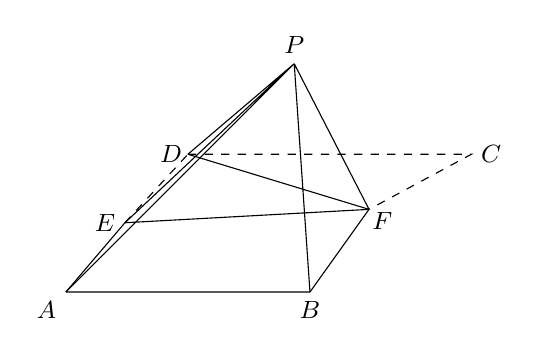
\begin{tikzpicture}[scale=1.0, font=\small]
  \coordinate (A) at (0,0);
  \coordinate (B) at (3.1,0);
  \coordinate (F) at (3.85,1.05);
  \coordinate (D) at (1.55,1.75);
  \coordinate (E) at (0.75,0.88);
  \coordinate (P) at (2.9,2.9);
  \coordinate (C) at (5.15,1.75);
  \draw (A) -- (B) -- (F);
  \draw (A) -- (E);
  \draw[dashed] (E) -- (D);
  \draw (D) -- (F);          % 折痕
  \draw (E) -- (F);
  \draw (A) -- (P)  (B) -- (P)  (F) -- (P)  (D) -- (P)  (E) -- (P);
  \draw[dashed] (D) -- (C) -- (F);
  \node[below left] at (A) {$A$};
  \node[below] at (B) {$B$};
  \node[below right, inner sep=1pt] at (F) {$F$};
  \node[left, inner sep=2pt] at (D) {$D$};
  \node[left] at (E) {$E$};
  \node[above] at (P) {$P$};
  \node[right] at (C) {$C$};
\end{tikzpicture}
\end{center}

\gksubpart{折叠问题的第一原则：分清"变"与"不变"}

\textbf{不变的}（在被折的 $\triangle DFC$ 内部）：$PF=CF$，$PD=CD$，$\angle DPF=\angle DCF=90^\circ$。

\textbf{不变的}（在留下的四边形 $ABFD$ 内部）：$AB$、$BF$、$FD$、$DE$、$EF$ 等一切长度与角度。

\textbf{变的}：$\triangle DFC$ 与底面的相对位置（这正是要靠已知条件 $PF\perp BF$ 来确定的）。

设正方形边长为 $2$，则 $BF=CF=1$，$EF=2$，$CD=2$，故折叠后

\[PF=1,\qquad PD=2\]

\gksubpart{(1) 证明平面 $PEF\perp$ 平面 $ABFD$}

\textbf{第一步：找底面内与 $BF$ 垂直的线。}

在原正方形中，$E$、$F$ 分别是 $AD$、$BC$ 的中点，故 $EF\parallel AB$。又 $AB\perp BC$，所以

\[EF\perp BC,\ \text{即}\ EF\perp BF\]

这条关系在折叠中\textbf{完全不受影响}（$E$、$F$、$B$ 都在没有被折动的部分里）。

\textbf{第二步：与已知条件联立。}

已知 $PF\perp BF$。又 $EF\perp BF$，且

\[EF\cap PF=F,\qquad EF,\ PF\subset\text{平面 }PEF\]

由\textbf{线面垂直的判定定理}：

\[BF\perp\text{平面 }PEF\]

\textbf{第三步：升级为面面垂直。}

$BF\subset$ 平面 $ABFD$，一条直线垂直于一个平面，则过这条直线的任何平面都垂直于该平面，故

\[\text{平面 }PEF\perp\text{平面 }ABFD\qquad\blacksquare\]

\gksubpart{(2) 求 $DP$ 与平面 $ABFD$ 所成角的正弦值}

由 (1) 已知 $BF\perp$ 平面 $PEF$，说明 $P$ 一定落在\textbf{过 $EF$ 且垂直于 $BF$ 的那个平面}内。据此建系最省事。

\textbf{建系}：以 $A$ 为原点，$AB$ 为 $x$ 轴，$AD$ 为 $y$ 轴，竖直向上为 $z$ 轴。则

\[A(0,0,0),\quad B(2,0,0),\quad F(2,1,0),\quad D(0,2,0),\quad E(0,1,0)\]

设 $P(x,y,z)$，$z>0$。三个条件：

1. \textbf{$PF\perp BF$}：$\overrightarrow{BF}=(0,1,0)$，$\overrightarrow{FP}=(x-2,\ y-1,\ z)$，
\[\overrightarrow{FP}\cdot\overrightarrow{BF}=y-1=0\ \Longrightarrow\ y=1\]
   （这正对应 (1) 中"$P$ 在过 $EF$ 的竖直平面内"。）

2. \textbf{$PF=1$}：$(x-2)^{2}+(y-1)^{2}+z^{2}=1$，代入 $y=1$ 得
\[(x-2)^{2}+z^{2}=1\]

3. \textbf{$PD=2$}：$x^{2}+(y-2)^{2}+z^{2}=4$，代入 $y=1$ 得
\[x^{2}+z^{2}=3\]

后两式相减：

\[x^{2}-(x-2)^{2}=2\ \Longrightarrow\ 4x-4=2\ \Longrightarrow\ x=\frac32\]

回代：$z^{2}=3-\dfrac94=\dfrac34$，取 $z=\dfrac{\sqrt3}2$。故

\[P\left(\frac32,\ 1,\ \frac{\sqrt3}2\right)\]

\textbf{求线面角。} 平面 $ABFD$ 就是 $z=0$ 平面，其法向量可取 $\boldsymbol n=(0,0,1)$。

\[\overrightarrow{DP}=\left(\frac32,\ 1-2,\ \frac{\sqrt3}2\right)=\left(\frac32,\ -1,\ \frac{\sqrt3}2\right)\]

\[|DP|=\sqrt{\frac94+1+\frac34}=\sqrt4=2\quad(\text{与 }PD=2\text{ 一致，验算通过})\]

线面角 $\theta$ 满足

\[\sin\theta=\frac{\left|\overrightarrow{DP}\cdot\boldsymbol n\right|}{|DP|\cdot|\boldsymbol n|}=\frac{\frac{\sqrt3}2}2=\frac{\sqrt3}4\]

\gkanswer{答案：$\dfrac{\sqrt3}4$}

\begin{gktip}
\textbf{方法提示}：翻折题最容易出错的地方是\textbf{把折叠前的关系当成折叠后还成立}。判断标准很简单：\textbf{这条关系涉及的点是否全在同一侧}（要么全在被折的部分，要么全在不动的部分）。$EF\perp BF$ 的三个点都在不动部分，所以能用；而"$PE$ 的长度"因为 $E$ 与 $P$ 分属两侧，折叠前的值就\textbf{不能}直接用了 —— 这正是本题必须靠 $PF\perp BF$ 建系求解的原因。

建系后用 $z$ 坐标除以 $|DP|$ 直接得线面角正弦，比找垂足、算射影快得多。
\end{gktip}

\par\medskip

\end{answer}
\begin{answer}
\gksolhead{19}{12 分，椭圆与角相等}

\textbf{题目}：椭圆 $C:\dfrac{x^{2}}2+y^{2}=1$ 右焦点 $F$，过 $F$ 的直线 $l$ 交 $C$ 于 $A$、$B$，$M(2,0)$。

\textbf{基本量}：$a^{2}=2$，$b^{2}=1$，$c^{2}=a^{2}-b^{2}=1$，故 $F(1,0)$。

\gksubpart{(1) 当 $l$ 与 $x$ 轴垂直时，求直线 $AM$ 的方程}

$l:x=1$ 代入椭圆：

\[\frac12+y^{2}=1\ \Longrightarrow\ y^{2}=\frac12\ \Longrightarrow\ y=\pm\frac{\sqrt2}2\]

取 $A\left(1,\dfrac{\sqrt2}2\right)$（$A$ 也可能是下面那个点，两种情形对称）。

\[k_{AM}=\frac{\frac{\sqrt2}2-0}{1-2}=-\frac{\sqrt2}2\]

直线 $AM$：

\[y=-\frac{\sqrt2}2(x-2)\]

若取 $A\left(1,-\dfrac{\sqrt2}2\right)$，则得 $y=\dfrac{\sqrt2}2(x-2)$。

\gkanswer{答案：$y=-\dfrac{\sqrt2}2(x-2)$ 或 $y=\dfrac{\sqrt2}2(x-2)$}

\gksubpart{(2) 证明 $\angle OMA=\angle OMB$}

\textbf{转化}：$M$ 在 $x$ 轴上，$O$ 也在 $x$ 轴上，所以 $\angle OMA$ 与 $\angle OMB$ 分别是 $MA$、$MB$ 与 $x$ 轴负方向的夹角。两角相等 $\iff$ $MA$ 与 $MB$ 关于 $x$ 轴对称 $\iff$

\[k_{MA}+k_{MB}=0\]

\textbf{情形一：$l$ 斜率不存在}（即 (1) 中的情形）。由对称性 $A$、$B$ 关于 $x$ 轴对称，结论显然成立。

\textbf{情形二：$l$ 斜率存在}，设 $l:y=k(x-1)$，$A\left(x_1,y_1\right)$，$B\left(x_2,y_2\right)$。

代入椭圆消 $y$：

\[\frac{x^{2}}2+k^{2}(x-1)^{2}=1\ \Longrightarrow\ x^{2}+2k^{2}(x-1)^{2}=2\]

\[\left(1+2k^{2}\right)x^{2}-4k^{2}x+\left(2k^{2}-2\right)=0\]

韦达定理：

\[x_1+x_2=\frac{4k^{2}}{1+2k^{2}},\qquad x_1x_2=\frac{2k^{2}-2}{1+2k^{2}}\]

\textbf{计算斜率之和}：

\[k_{MA}+k_{MB}=\frac{y_1}{x_1-2}+\frac{y_2}{x_2-2}=\frac{k\left(x_1-1\right)}{x_1-2}+\frac{k\left(x_2-1\right)}{x_2-2}\]

通分，分子为

\[k\left[\left(x_1-1\right)\left(x_2-2\right)+\left(x_2-1\right)\left(x_1-2\right)\right]\]

展开括号内：

\[\left(x_1x_2-2x_1-x_2+2\right)+\left(x_1x_2-2x_2-x_1+2\right)=2x_1x_2-3\left(x_1+x_2\right)+4\]

代入韦达：

\[2\cdot\frac{2k^{2}-2}{1+2k^{2}}-3\cdot\frac{4k^{2}}{1+2k^{2}}+4=\frac{\left(4k^{2}-4\right)-12k^{2}+4\left(1+2k^{2}\right)}{1+2k^{2}}\]

\[=\frac{4k^{2}-4-12k^{2}+4+8k^{2}}{1+2k^{2}}=\frac{0}{1+2k^{2}}=0\]

\textbf{分子恒为 $0$}（与 $k$ 无关），而分母 $\left(x_1-2\right)\left(x_2-2\right)\ne0$（因为 $|x|\le\sqrt2<2$），故

\[k_{MA}+k_{MB}=0\]

所以 $MA$ 与 $MB$ 的倾斜角互补，$\angle OMA=\angle OMB$。$\blacksquare$

\begin{gktip}
\textbf{方法提示}：这是圆锥曲线中的\textbf{定点/定值问题}，标准打法是"\textbf{设而不求 + 韦达定理 + 目标式化简后系数恒为零}"。

值得注意的是点 $M(2,0)$ 的来历：$x=2$ 正是椭圆的\textbf{右准线} $x=\dfrac{a^{2}}c=\dfrac21=2$。"从准线上一点看焦点弦两端张角相等"是椭圆的一条一般性质，本题是它的特例。
\end{gktip}

\par\medskip

\end{answer}
\begin{answer}
\gksolhead{20}{12 分，二项分布与决策}

\textbf{题目}：见试题。

\gksubpart{(1) 求 $f(p)$ 的最大值点 $p_0$}

$20$ 件中恰有 $2$ 件不合格，服从二项分布：

\[f(p)=C_{20}^{2}p^{2}(1-p)^{18},\qquad p\in(0,1)\]

\textbf{求导}（$C_{20}^{2}=190$ 是常数，可提出）：

\[f'(p)=C_{20}^{2}\left[2p(1-p)^{18}-18p^{2}(1-p)^{17}\right]\]

提取公因式 $p(1-p)^{17}$：

\[f'(p)=C_{20}^{2}\,p(1-p)^{17}\left[2(1-p)-18p\right]=C_{20}^{2}\,p(1-p)^{17}(2-20p)\]

在 $(0,1)$ 上 $p>0$、$(1-p)^{17}>0$，故 $f'$ 的符号由 $2-20p$ 决定：

\begin{itemize}
\item $p<0.1$ 时 $f'>0$，$f$ 递增；
\item $p>0.1$ 时 $f'<0$，$f$ 递减。
\end{itemize}

\gkanswer{答案：$p_0=0.1$}

\begin{gktip}
这其实就是\textbf{极大似然估计}：观测到 $20$ 件里有 $2$ 件不合格，最"像"的不合格率就是 $\dfrac2{20}=0.1$。
\end{gktip}

\gksubpart{(2) 决策}

取 $p=p_0=0.1$。

\gksubpart{① 求 $EX$}

若\textbf{不检验}余下的 $180$ 件：

\begin{itemize}
\item \textbf{检验费}：只检验了 $20$ 件，$20\times2=40$ 元（这是常数）；
\item \textbf{赔偿费}：余下 $180$ 件中的不合格品会流入用户手中。设其中不合格品数为 $Y$，则
\end{itemize}
\[Y\sim B(180,\ 0.1),\qquad EY=180\times0.1=18\]
  赔偿费为 $25Y$。

于是

\[X=40+25Y\]

由期望的线性性：

\[EX=40+25\,EY=40+25\times18=40+450=490\ (\text{元})\]

\gksubpart{② 是否该检验余下产品}

若\textbf{检验}余下的 $180$ 件：全部 $200$ 件都要检验，且不合格品会被换成合格品，不产生赔偿：

\[\text{总费用}=200\times2=400\ (\text{元})\]

这是一个\textbf{确定值}（不是随机变量），其期望就是 $400$。

比较两个方案的期望费用：

\[400<490\]

\textbf{结论：应该对这箱余下的所有产品作检验}（期望费用更低，可省约 $90$ 元）。

\begin{gktip}
\textbf{方法提示}：本题第 (2) 问的关键是\textbf{别忘了已经花掉的 $40$ 元检验费}。另外要理解"检验后更换为合格品"意味着检验能\textbf{完全消除}赔偿风险，所以方案二的费用是确定的 $400$ 元，不需要再算期望。
\end{gktip}

\par\medskip

\end{answer}
\begin{answer}
\gksolhead{21}{12 分，导数压轴}

\textbf{题目}：$f(x)=\dfrac1x-x+a\ln x$（定义域 $x>0$）。

\gksubpart{(1) 讨论 $f(x)$ 的单调性}

\[f'(x)=-\frac1{x^{2}}-1+\frac ax=\frac{-1-x^{2}+ax}{x^{2}}=-\frac{x^{2}-ax+1}{x^{2}}\]

因 $x^{2}>0$，$f'$ 的符号与 $g(x)=x^{2}-ax+1$ \textbf{相反}。

判别式 $\Delta=a^{2}-4$。

\textbf{情形一：$a\le2$。}

\begin{itemize}
\item 若 $-2\le a\le2$：$\Delta\le0$，$g(x)\ge0$ 恒成立；
\item 若 $a<-2$：$g$ 的对称轴 $x=\dfrac a2<-1<0$，而定义域是 $x>0$，故在定义域上 $g$ 单调递增，$g(x)>g(0)=1>0$。
\end{itemize}

两种情况下都有 $g(x)\ge0$，故 $f'(x)\le0$：

\textbf{$f(x)$ 在 $(0,+\infty)$ 上单调递减。}

\textbf{情形二：$a>2$。}

$\Delta>0$，$g$ 有两个不同实根

\[x_1=\frac{a-\sqrt{a^{2}-4}}2,\qquad x_2=\frac{a+\sqrt{a^{2}-4}}2\]

由韦达定理 $x_1+x_2=a>0$，$x_1x_2=1>0$，故\textbf{两根均为正数}，都在定义域内，且 $0<x_1<1<x_2$。

$g$ 开口向上：在 $\left(x_1,x_2\right)$ 内 $g<0$，其余 $g>0$。因 $f'$ 与 $g$ 反号：

\begin{itemize}
\item $f(x)$ 在 $\left(0,x_1\right)$ 上\textbf{单调递减}；
\item $f(x)$ 在 $\left(x_1,x_2\right)$ 上\textbf{单调递增}；
\item $f(x)$ 在 $\left(x_2,+\infty\right)$ 上\textbf{单调递减}。
\end{itemize}

\gksubpart{(2) 证明 $\dfrac{f\left(x_1\right)-f\left(x_2\right)}{x_1-x_2}<a-2$}

由 (1) 知，存在两个极值点当且仅当 $a>2$，且

\[x_1+x_2=a,\qquad x_1x_2=1\]

\textbf{第一步：化简差商。}

\[f\left(x_1\right)-f\left(x_2\right)=\left(\frac1{x_1}-\frac1{x_2}\right)-\left(x_1-x_2\right)+a\left(\ln x_1-\ln x_2\right)\]

第一个括号利用 $x_1x_2=1$：

\[\frac1{x_1}-\frac1{x_2}=\frac{x_2-x_1}{x_1x_2}=x_2-x_1=-\left(x_1-x_2\right)\]

于是

\[f\left(x_1\right)-f\left(x_2\right)=-2\left(x_1-x_2\right)+a\left(\ln x_1-\ln x_2\right)\]

两边同除以 $x_1-x_2$（$\ne0$）：

\[\frac{f\left(x_1\right)-f\left(x_2\right)}{x_1-x_2}=-2+a\cdot\frac{\ln x_1-\ln x_2}{x_1-x_2}\]

\textbf{第二步：把目标不等式化简。} 要证它 $<a-2$，即证

\[a\cdot\frac{\ln x_1-\ln x_2}{x_1-x_2}<a\]

由 $a>2>0$，两边同除 $a$，只需证

\[\frac{\ln x_1-\ln x_2}{x_1-x_2}<1\]

\textbf{第三步：证明这个不等式。} 不妨设 $x_1<x_2$（由 $x_1x_2=1$ 知 $0<x_1<1<x_2$）。此时 $x_1-x_2<0$，不等式\textbf{变号}为

\[\ln x_1-\ln x_2>x_1-x_2\]

\textbf{第四步：换元。} 由 $x_1x_2=1$ 可设

\[x_1=s,\qquad x_2=\frac1s,\qquad s\in(0,1)\]

代入要证的式子：

\[\ln s-\ln\frac1s>s-\frac1s\ \Longleftrightarrow\ 2\ln s-s+\frac1s>0\]

\textbf{第五步：构造函数。} 令

\[h(s)=2\ln s-s+\frac1s,\qquad s\in(0,1)\]

求导：

\[h'(s)=\frac2s-1-\frac1{s^{2}}=\frac{2s-s^{2}-1}{s^{2}}=-\frac{(s-1)^{2}}{s^{2}}\le0\]

且仅在 $s=1$ 处取等，故 $h$ 在 $(0,1]$ 上\textbf{严格单调递减}。又

\[h(1)=2\ln1-1+1=0\]

所以对一切 $s\in(0,1)$：

\[h(s)>h(1)=0\]

这正是第四步所需的不等式。逐步回溯，原不等式成立。$\blacksquare$

\begin{gktip}
\textbf{方法提示}：本题是导数压轴的经典结构，三个关键动作：

1. \textbf{韦达定理提取两个极值点的关系}（$x_1x_2=1$ 是本题的灵魂，它让 $\dfrac1{x_1}-\dfrac1{x_2}$ 直接变成 $-\left(x_1-x_2\right)$）；
2. \textbf{把含两个变量的不等式化成一个变量}（这里用 $x_2=\dfrac1{x_1}$ 换元，是"极值点偏移"类问题的通用手法）；
3. \textbf{构造函数 $h$ 并证明其单调性}，通常导数会恰好凑成完全平方 —— 本题 $h'(s)=-\dfrac{(s-1)^{2}}{s^{2}}$ 就是这样。

若在第三步忘了"除以负数要变号"，后面的推导会全部反向，这是本题最常见的失分点。
\end{gktip}

\par\medskip

\end{answer}
\gkpart{选考题（现行考纲已取消，仅存档）}

\begin{answer}
\gksolhead{22}{10 分，坐标系与参数方程}

\textbf{题目}：$C_1:y=k|x|+2$；$C_2:\rho^{2}+2\rho\cos\theta-3=0$。

\gksubpart{(1) 求 $C_2$ 的直角坐标方程}

利用 $\rho^{2}=x^{2}+y^{2}$，$\rho\cos\theta=x$：

\[x^{2}+y^{2}+2x-3=0\]

配方：

\[(x+1)^{2}+y^{2}=4\]

这是\textbf{圆心 $(-1,0)$、半径 $2$ 的圆}。

\gksubpart{(2) 若 $C_1$ 与 $C_2$ 有且仅有三个公共点，求 $C_1$ 的方程}

\textbf{认清 $C_1$ 的形状}：$y=k|x|+2$ 由两条射线拼成，顶点为 $(0,2)$：

\[\text{右支：}y=kx+2\ (x\ge0);\qquad \text{左支：}y=-kx+2\ (x\le0)\]

顶点 $(0,2)$ 到圆心 $(-1,0)$ 的距离为 $\sqrt{1+4}=\sqrt5>2$，故\textbf{顶点在圆外}。

\textbf{为什么必须"一支相切、一支两交点"}：每条射线与圆最多 $2$ 个交点，两支合计要凑出 $3$ 个，只能是 $2+1$。而 $1$ 个交点有两种可能 —— 相切，或者射线端点截断后只剩一个交点。由于顶点 $(0,2)$ 在圆外，端点截断不会产生"恰好一个"的情形，故必为\textbf{相切}。

\textbf{先定符号}：若 $k>0$（开口向上），两支都向上远离圆（圆的最高点是 $y=2$，仅在 $x=-1$ 处），右支完全在圆外，左支最多 $2$ 个交点，凑不出 $3$ 个。故 $k<0$（开口向下）。

\textbf{尝试右支相切}：右支所在直线 $kx-y+2=0$，圆心 $(-1,0)$ 到它的距离为半径 $2$：

\[\frac{|-k-0+2|}{\sqrt{k^{2}+1}}=2\ \Longrightarrow\ (2-k)^{2}=4\left(k^{2}+1\right)\]

\[4-4k+k^{2}=4k^{2}+4\ \Longrightarrow\ 3k^{2}+4k=0\ \Longrightarrow\ k=0\ \text{或}\ k=-\frac43\]

$k=0$ 时 $C_1$ 退化为直线 $y=2$，与圆只有 $1$ 个公共点，舍去。取 $k=-\dfrac43$。

\textbf{验证 $k=-\dfrac43$}：

\begin{itemize}
\item 右支 $y=-\dfrac43x+2$ 即 $4x+3y-6=0$，圆心距 $\dfrac{|-4-6|}5=2$  相切。
\end{itemize}
  切点：$(-1,0)+2\cdot\dfrac{(4,3)}5=\left(\dfrac35,\dfrac65\right)$，横坐标 $\dfrac35\ge0$  \textbf{确实在右支上}。
\begin{itemize}
\item 左支 $y=\dfrac43x+2$ 即 $4x-3y+6=0$，圆心距 $\dfrac{|-4+6|}5=\dfrac25<2$，相交于两点。
\end{itemize}
  联立解得 $25x^{2}+66x+9=0$，$x=\dfrac{-33\pm12\sqrt6}{25}\approx-0.14,\ -2.50$，两个都 $\le0$  \textbf{确实都在左支上}。

共 $3$ 个公共点 

\textbf{尝试左支相切}：直线 $kx+y-2=0$，距离为 $2$ 给出 $3k^{2}-4k=0$，即 $k=0$ 或 $k=\dfrac43$，与 $k<0$ 矛盾，无解。

\gkanswer{答案：$C_1:y=-\dfrac43|x|+2$}

\begin{gktip}
\textbf{方法提示}：这类题\textbf{必须验证切点/交点是否落在射线的定义域内}。相切只保证直线与圆相切，但射线只是直线的一半，如果切点在被截掉的那一半上，公共点数就对不上了。本题两次验证都通过，属于"运气好"，但考场上不验证就是赌博。
\end{gktip}

\par\medskip

\end{answer}
\begin{answer}
\gksolhead{23}{10 分，绝对值不等式}

\textbf{题目}：$f(x)=|x+1|-|ax-1|$。

\gksubpart{(1) 当 $a=1$ 时，求 $f(x)>1$ 的解集}

\[f(x)=|x+1|-|x-1|\]

以 $-1$ 和 $1$ 为分界点分三段讨论：

\textbf{① $x<-1$}：$|x+1|=-(x+1)$，$|x-1|=-(x-1)$，

\[f(x)=-(x+1)+(x-1)=-2\]

$-2>1$ 不成立，此段无解。

\textbf{② $-1\le x<1$}：$|x+1|=x+1$，$|x-1|=-(x-1)$，

\[f(x)=(x+1)+(x-1)=2x\]

$2x>1\Rightarrow x>\dfrac12$。与本段范围求交：$\dfrac12<x<1$。

\textbf{③ $x\ge1$}：$|x+1|=x+1$，$|x-1|=x-1$，

\[f(x)=(x+1)-(x-1)=2\]

$2>1$ 恒成立，此段全部满足：$x\ge1$。

合并 ②③：

\[\left(\frac12,1\right)\cup[1,+\infty)=\left(\frac12,+\infty\right)\]

\gkanswer{答案：$\left\{x\ \middle|\ x>\dfrac12\right\}$}

\begin{gktip}
\textbf{几何解释}：$|x+1|-|x-1|$ 表示"$x$ 到 $-1$ 的距离减去到 $1$ 的距离"，它在 $[-1,1]$ 上线性地从 $-2$ 增到 $2$，两侧则为常数。
\end{gktip}

\gksubpart{(2) 若 $x\in(0,1)$ 时 $f(x)>x$ 成立，求 $a$ 的取值范围}

\textbf{关键简化}：$x\in(0,1)$ 时 $x+1>0$，故 $|x+1|=x+1$。不等式变为

\[x+1-|ax-1|>x\ \Longleftrightarrow\ |ax-1|<1\]

去绝对值：

\[-1<ax-1<1\ \Longleftrightarrow\ 0<ax<2\]

要求这对\textbf{所有} $x\in(0,1)$ 成立。

\textbf{左边 $ax>0$}：因 $x>0$，等价于 $a>0$。

\textbf{右边 $ax<2$}：因 $a>0$，$ax$ 关于 $x$ 单调递增，在 $x\in(0,1)$ 上的上确界为 $a\cdot1=a$（取不到）。故只需

\[a\le2\]

（$a=2$ 时 $ax<2$ 对开区间内所有 $x$ 严格成立，可以取到。）

\gkanswer{答案：$a\in(0,2]$}

\begin{gktip}
\textbf{方法提示}：本题的漂亮之处在于 $|x+1|$ 与右边的 $x$ \textbf{恰好抵消}，把一个含参绝对值不等式化成极简的 $|ax-1|<1$。看到区间限制 $x\in(0,1)$ 就应该先判断各绝对值内部的符号 —— 这一步做对了，题就做完一半。

端点 $a=2$ 能否取到，取决于 $x$ 的区间是开还是闭：这里 $x\in(0,1)$ 是开区间，$x$ 取不到 $1$，所以 $ax<2$ 恒成立，$a=2$ 合法。若改成 $x\in(0,1]$，答案就要变成 $(0,2)$。
\end{gktip}

\par\medskip


\end{answer}